\documentclass[12pt] {article}

%%% Preambuła %%%
\usepackage[T1]{fontenc}
\usepackage[polish]{babel}
\usepackage[utf8]{inputenc}
\usepackage{lmodern}
\usepackage{hyperref}
\usepackage{mathptmx}
\usepackage{float}
\usepackage{graphicx}
\usepackage{amsmath}
\usepackage{xcolor}
\usepackage{listings}
\selectlanguage{polish}

\usepackage{geometry}

\geometry{
 a4paper,
 total={170mm,257mm},
 left=20mm,
 top=20mm,
 }


%%% Ustawienia listingów %%%
\definecolor{vgreen}{RGB}{104,180,104}
\definecolor{vblue}{RGB}{49,49,255}
\definecolor{vorange}{RGB}{255,143,102}

\lstdefinestyle{verilog-style}
{
    language=Verilog,
    basicstyle=\small\ttfamily,
    keywordstyle=\color{vblue},
    identifierstyle=\color{black},
    commentstyle=\color{vgreen},
	frame=single,
    tabsize=8,
    moredelim=*[s][\colorIndex]{[}{]},
    literate=*{:}{:}1
}

\makeatletter
\newcommand*\@lbracket{[}
\newcommand*\@rbracket{]}
\newcommand*\@colon{:}
\newcommand*\colorIndex{%
    \edef\@temp{\the\lst@token}%
    \ifx\@temp\@lbracket \color{black}%
    \else\ifx\@temp\@rbracket \color{black}%
    \else\ifx\@temp\@colon \color{black}%
    \else \color{vorange}%
    \fi\fi\fi
}
\makeatother


%%% Strona tytułowa %%%
\title {
	Języki Opisu Sprzętu \\
	\large Projekt: Elektroniczny Sejf Hotelowy \\
	Dokumentacja}

\author {
	Arkadiusz Kasprzak \\
	Jarosław Cierpich \\
	Wydział Fizyki i Informatyki Stosowanej \\ 
	Informatyka Stosowana}

	
\begin{document}

\begin{figure}
\centering

\includegraphics[scale = 1.5]{res/agh_znk_wbr_cmyk}
\end{figure}

%%% Strona tytułowa %%%
\maketitle

%%% Spis treści %%%
\newpage
\tableofcontents

\newpage
\section{Wstęp}
Niniejszy dokument stanowi dokumentację projektu \textbf{Elektroniczny Sejf Hotelowy} wykonanego w ramach przedmiotu \textbf{Języki Opisu Sprzętu} (WFiIS AGH) przez Jarosława Cierpicha i Arkadiusza Kasprzaka. Dokument ten zawiera m.in. założenia projektowe oraz opis wymaganej funkcjonalności, dokumentację przeznaczoną dla użytkownika projektu, dokumentację techniczną, analizę procesu syntezy oraz opis procedury testowania.

\section{Projekt}
Ten rozdział poświęcony został opisowi założeń projektowych oraz wymaganej funkcjonalności.

\subsection{Założenia projektowe}

\subsection{Wymagana funkcjonalność}

\section{Dokumentacja użytkownika}

\section{Dokumentacja techniczna}
\subsection{Warstwa Hardware}
\subsection{Warstwa Software - architektura}
\subsection{Warstwa Software - moduły projektu}

\section{Analiza procesu syntezy}

\section{Testy}
Ostatni rozdział poświęcony został procesowi testowania projektu - w tym przygotowanym modułom testowym oraz procesowi testowania manualnego. 

\subsection{Moduły testujące}
Projekt zawiera \textbf{TUTAJ WSTAWIC ILE} modułów testowych (tzw. moduły \textit{Testbench}). Umożliwiają one przeprowadzenie symulacji działania modułów projektu. Moduły testowane były za pomocą dwóch typów symulacji:
\begin{itemize}
\item symulacja behawioralna (\textit{behavioral simulation})
\item symulacja po syntezie z uwzględnieniem parametrów czasowych (\textit{post-synthesis timing simulation})
\end{itemize}
\textbf{TUTAJ WSTAWIC STRUKTURE TB}
Podstawowa struktura większości modułów \textit{Testbench} jest podobna - składają się one z:
\begin{itemize}
\item deklaracji parametrów wejściowych modułu (jeśli takie są)
\item deklaracji zmiennych stanowiących wejścia i wyjścia testowanego modułu oraz zmiennej odpowiadającej za \textit{Global System Reset - GSR}
\item instancji testowanego modułu (\textit{UUT - Unit Under Test})
\item generacji sygnałów wejściowych testowanego modułu (w tym zwykle sygnału zegara i resetu)
\end{itemize}
Listing \ref{lst:testy} ilustruje opisaną powyżej strukturę.

\begin{lstlisting}[style={verilog-style}, caption={Uproszczona struktura wykonanych modułów testujących}, label={lst:testy}]
module TbExample();
    
    // parametry    
    localparam mod = 3;    
    
    // wejscia
    reg clk, rst;
    reg in1;
    
    // wyjscia
    reg [3:0] out1; 
    
    // ...

    // GSR - Global System Reset
    wire gsr = glbl.GSR;

    // UUT - Unit Under Test
    ExampleModule #(.mod(mod)) EXAMPLE (
        .clk(clk), .rst(rst), .in1(in1), .out1(out1));

    // generacja sygnalow wejsciowych

    // zegar
    initial begin
        clk = 1'b0;
        @(negedge gsr);
        forever #5 clk = ~clk;
    end
    
    // reset
    initial begin
        rst = 1'b1;
        @(negedge gsr);
        #5 rst = 1'b0;
    end
    
    // in1
    initial begin 
        // kod generujacy wartosci sygnalu in1
    end
    
    // ...
    
endmodule
\end{lstlisting}

W dalszej części tego podrozdziału omówione zostaną poszczególne moduły testujące oraz wyniki przeprowadzonych symulacji behawioralnych. 

\subsubsection{Testy modułu Bcd2Dec}


\begin{figure}[H]
\centering
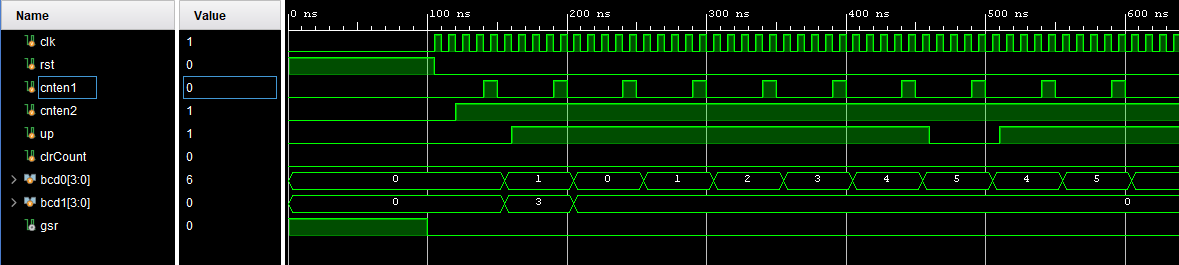
\includegraphics[width=\textwidth]{res/behav_sims/Bcd2Dec_behavSim_1.png}
\caption{Tutaj dac opis}
\end{figure}

\begin{figure}[H]
\centering
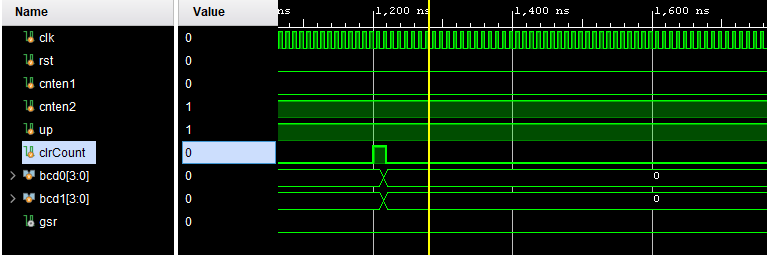
\includegraphics[width=\textwidth]{res/behav_sims/Bcd2Dec_behavSim_2.png}
\caption{Tutaj dac opis}
\end{figure}


\subsubsection{Testy modułu ClkDiv}

\subsection{Testy manualne}



\end{document}